\chapter{Tampilan Aplikasi Digital Wellbeing}
\label{chpt:gambar_dw}

\begin{figure}[h]
  \centering
  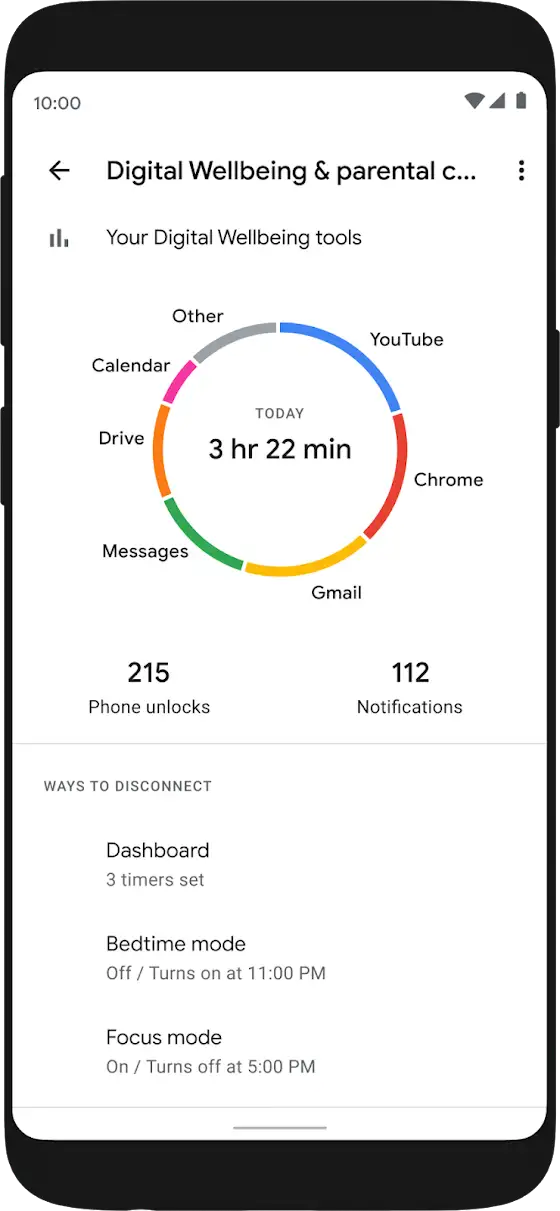
\includegraphics[width=0.25\textwidth]{appendix-a-dashboard.png}
  \caption{Fitur Dashboard pada aplikasi Digital Wellbeing (Android, 2019)}
\end{figure}

\begin{figure}[h]
  \centering
  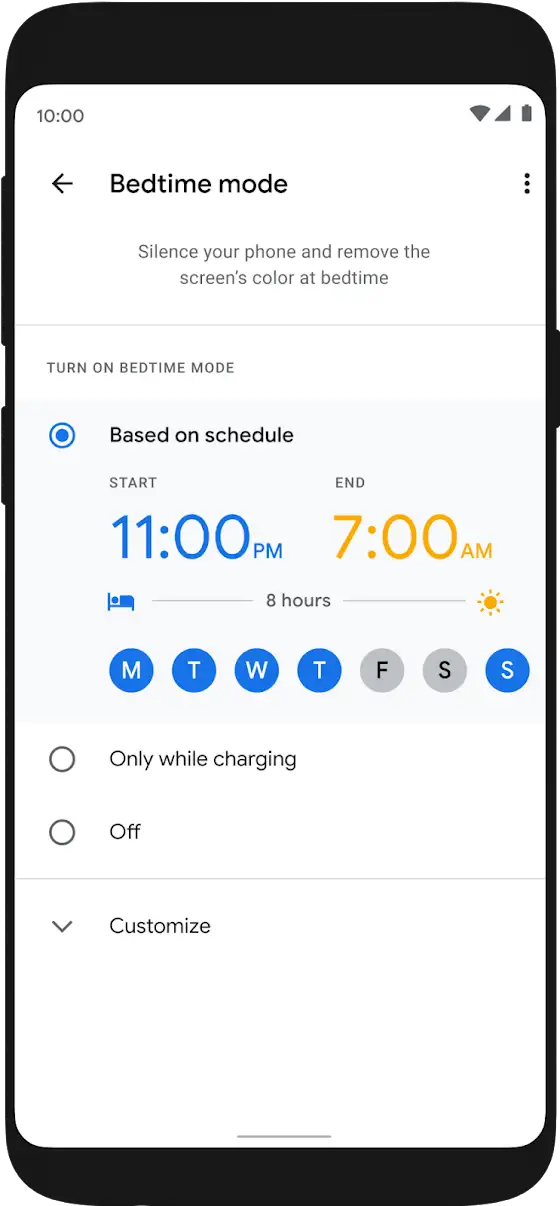
\includegraphics[width=0.25\textwidth]{appendix-a-bedtime-mode.png}
  \caption{Fitur Bedtime Mode pada aplikasi Digital Wellbeing (Android, 2019)}
\end{figure}

\begin{figure}[h]
  \centering
  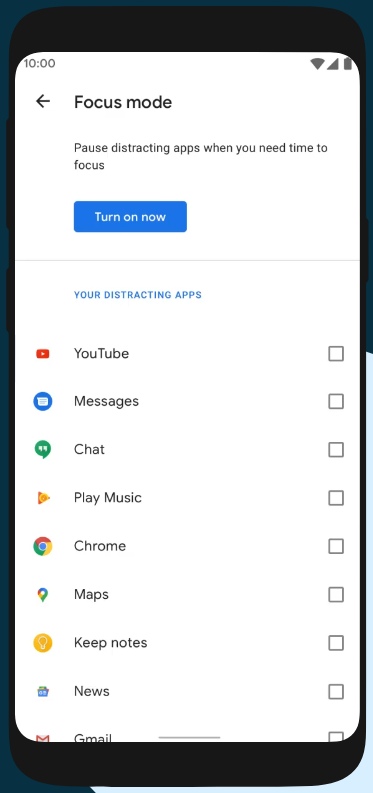
\includegraphics[width=0.25\textwidth]{appendix-a-focus-mode-1.png}
  \caption{Fitur Focus Mode pada aplikasi Digital Wellbeing, halaman pengaturan (Android, 2019)}
\end{figure}

\begin{figure}[h]
  \centering
  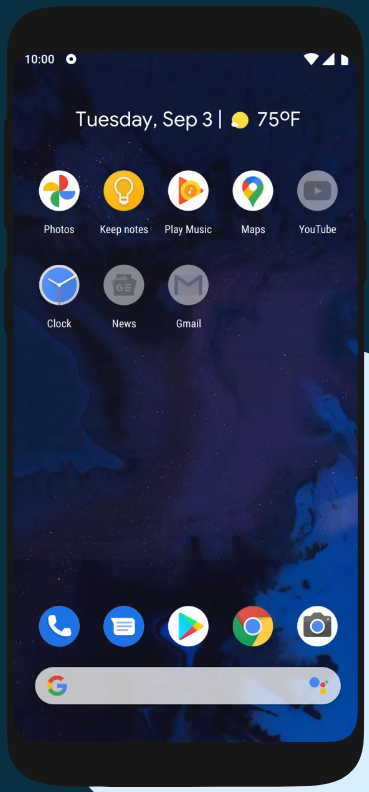
\includegraphics[width=0.25\textwidth]{appendix-a-focus-mode-2.png}
  \caption{Fitur Focus Mode pada aplikasi Digital Wellbeing, mengubah warna ikon aplikasi menjadi berskala abu-abu (Android, 2019)}
\end{figure}

\begin{figure}[h]
  \centering
  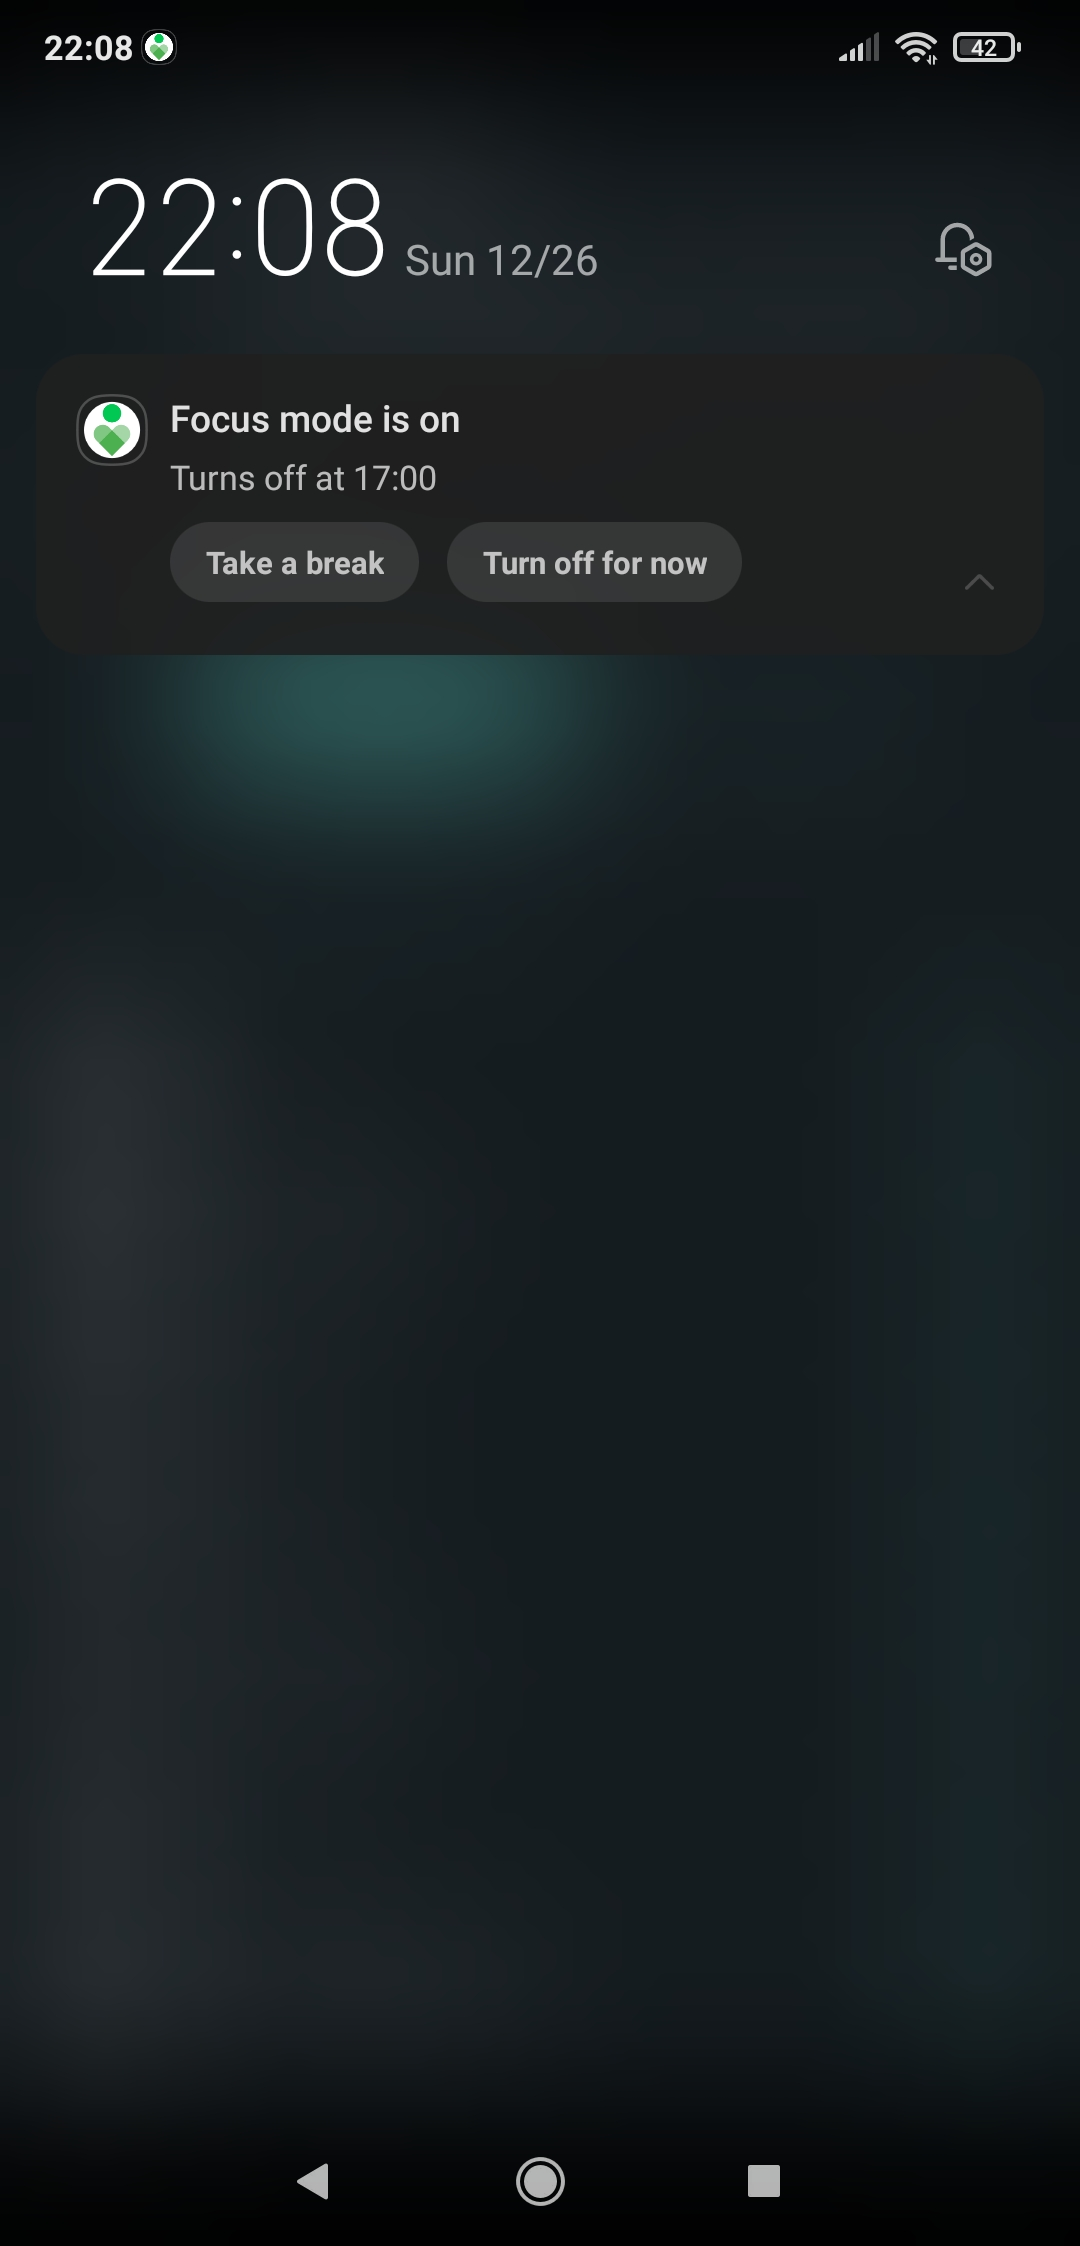
\includegraphics[width=0.25\textwidth]{appendix-a-focus-mode-3.jpg}
  \caption{Fitur Focus Mode pada aplikasi Digital Wellbeing, notifikasi status aktif}
\end{figure}

\begin{figure}[h]
  \centering
  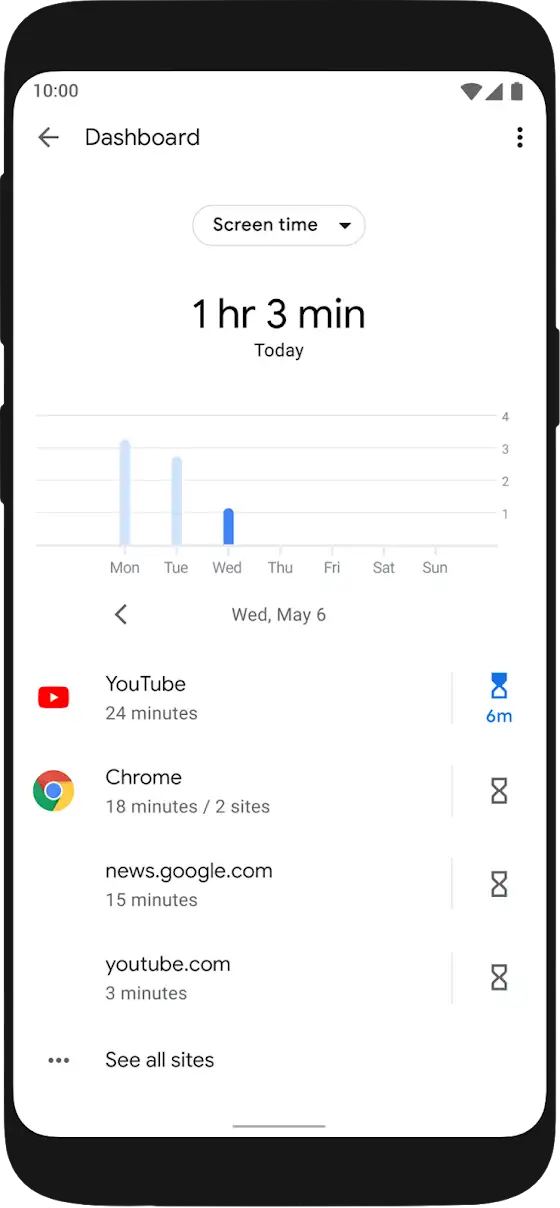
\includegraphics[width=0.25\textwidth]{appendix-a-app-timer.png}
  \caption{Fitur App Timers pada aplikasi Digital Wellbeing (Android, 2019)}
\end{figure}
